\section{The Real-Time Adaptive Loop}
\label{sec:design-loop}
% Authoring brief for this section lives in section.md (§5.4).
\Cref{sec:design-modules} described the four concerns as a static structure of ports and dependencies.
This section sets that structure in motion, as the loop that runs throughout a live reading session, and confronts the concessions that liveness imposes on the clean separation just established.
The loop is where the responsiveness driver D2 and the robustness driver D3 are met, and where they stand in their sharpest tension with the modularity of D1.

One adaptive cycle proceeds in the order of the data, and \cref{fig:design-loop} traces it across the parties involved.
A gaze sample originates at the eye tracker and reaches the core, which mirrors it on the dedicated real-time channel to the participant's reading surface and to the researcher's console, the second screen introduced in \cref{sec:design-style} that mirrors the reading surface and carries the session controls.
The participant's reading surface, which alone knows the rendered layout, maps the sample to a position in the text and returns an enriched observation to the core.
The core's analysis layer projects the stream of observations into oculomotor events, and a change in that analysed state triggers the decision layer to evaluate, drawing on either the built-in strategy or an external provider.
Those analysed events are rendered on the console, which overlays the mirrored text with a fixation heat map and the recent saccades, so that the researcher observes not only where but how the participant is reading.
The decision yields at most one intervention proposal, which is either applied at once or, in advisory operation, surfaced on the console for the researcher to approve or reject, informed by those overlays, and committed only on approval.
Applying it produces an adapted view and an intervention event, which the core returns to the participant's reading surface to re-render and mirrors to the console, closing the cycle.

\begin{figure}[htbp]
\centering
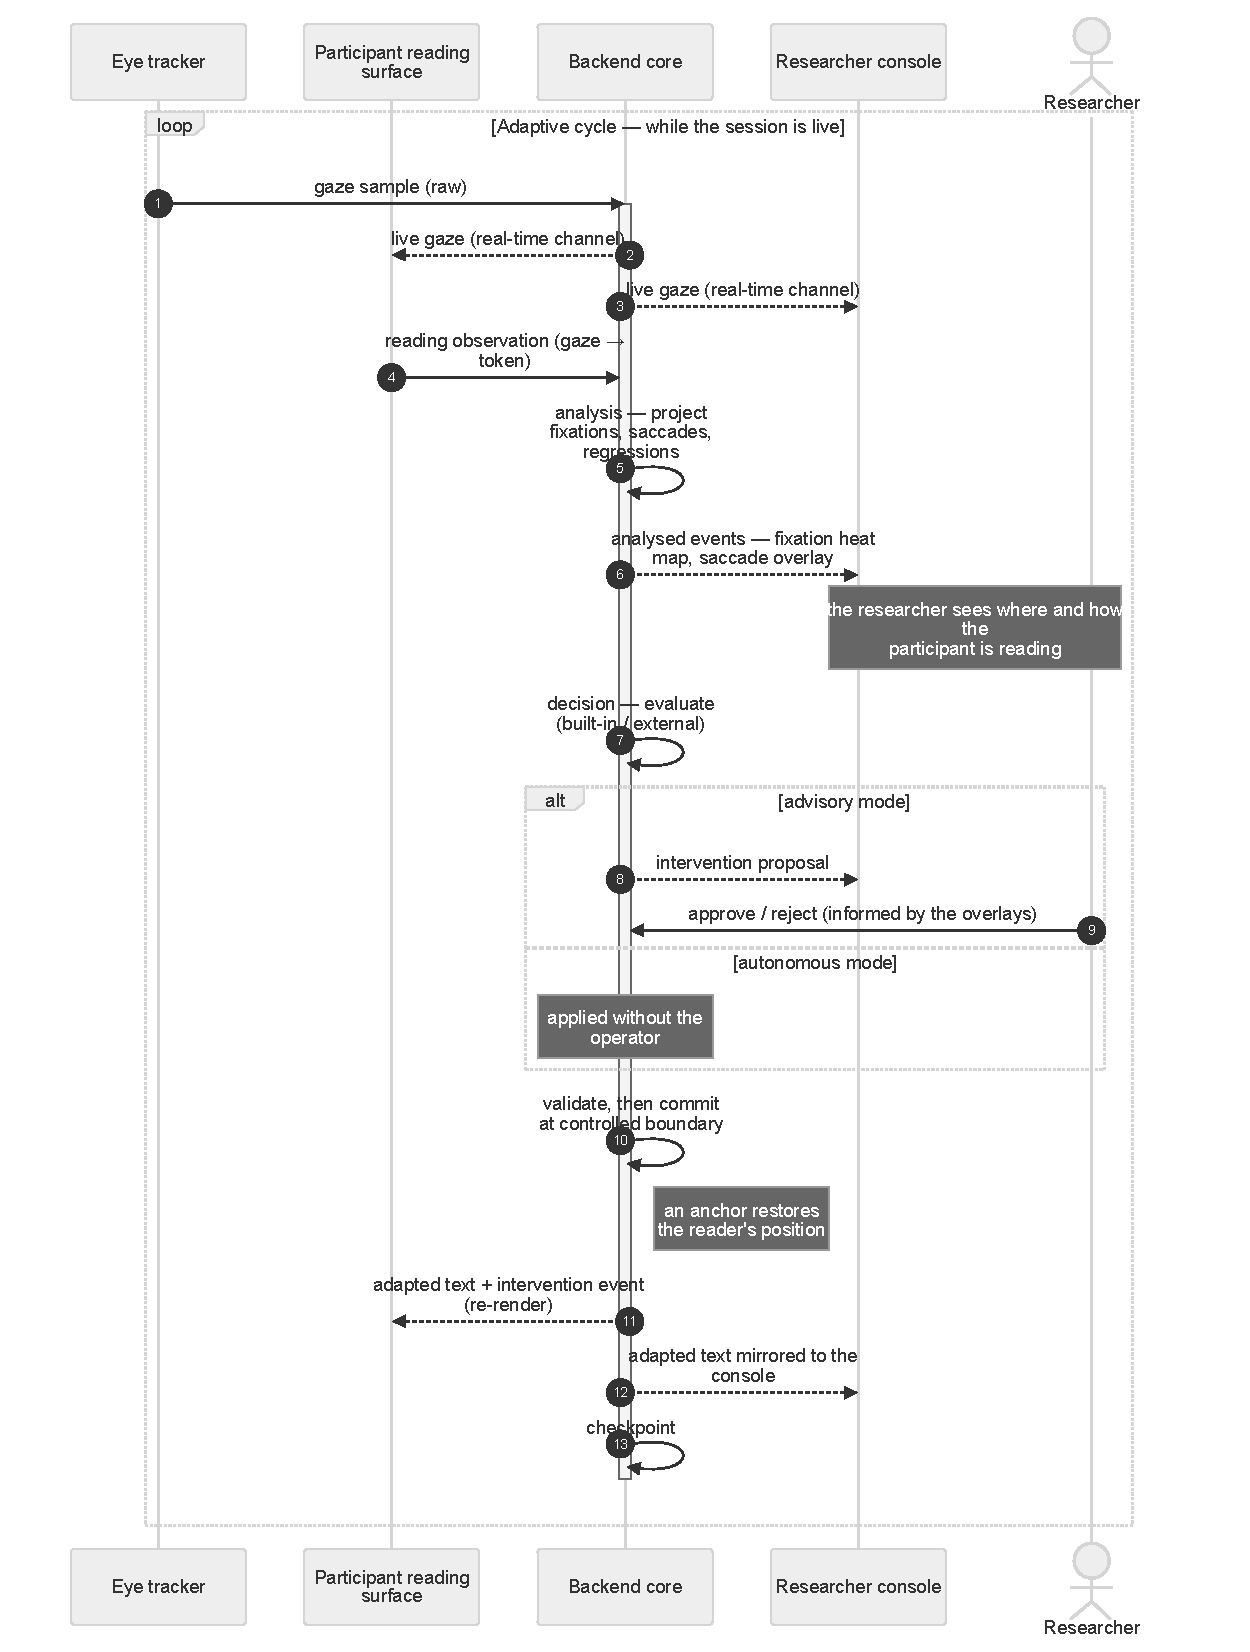
\includegraphics[width=\linewidth]{Chapters/05_SystemDesign/adaptive-loop.pdf}
\caption{One iteration of the real-time adaptive loop across the two front-end surfaces. High-frequency gaze is mirrored on the dedicated real-time channel to both the participant's reading surface and the researcher's console; the reading surface returns a content-anchored observation; the core projects oculomotor events (fixations, saccades, and regressions) and renders them on the console as a fixation heat map and a saccade overlay, so that the researcher can read the participant's behaviour. The core then evaluates a decision (using the built-in strategy or an external provider) and, in advisory mode, awaits researcher approval before validating and committing the intervention at a controlled boundary; the adapted text is returned to the reading surface and mirrored to the console. The self-calls on the backend core denote the analysis, decision, intervention, and persistence steps performed within it, and the checkpoint is written on a best-effort basis.}
\label{fig:design-loop}
\end{figure}

The cycle just described conceals a deliberate split in timescale that is the key to meeting the responsiveness budget D2.
High-frequency gaze does not travel the request and response path used for commands and setup; it flows on a separate real-time channel, so that mirroring a sample to the reading surface and the console never waits on the slower control path.
On that hot path the core does the minimum: it sanitises the sample, retains it as the latest value, and broadcasts it, without acquiring the lock that guards session lifecycle and decision state.
The heavier modular pipeline of analysis, decision, and intervention runs at the cadence of analysed-state changes rather than once per raw sample, so the indirection introduced for modularity in \cref{sec:design-modules} is kept off the per-sample path.
The end-to-end latency that this arrangement must respect, from gaze to committed intervention, is the budget evaluated in \cref{ch:evaluation} under RQ2.

This split is the architecture's answer to a tension we do not wish to hide.
The cleanest per-concern indirection is rarely the fastest at runtime, and an intervention delivered after the moment at which it remains valid is of no use to the reader.
We reconcile separation with speed not by diluting the contracts of \cref{sec:design-modules} but by confining their indirection to the lower-frequency control path, leaving the sensing path thin and direct.

Where an intervention is committed matters as much as when, because a typographic change alters the very layout the participant is reading.
The intervention contract is therefore two-phase: a proposal is first validated against the current reading context and only then committed, and the commit is performed at a controlled boundary rather than at an arbitrary instant (D7).
Each commit carries an anchor, a sentence, token, or block together with a measured anchor error and the viewport displacement, so that the reading surface can restore the reader's position across the change.
This commit discipline is the architectural expression of the recovery concern reported in the literature \cite{jensen2025context}: it is what allows a micro-intervention to adapt the text without costing the participant their place, which is the property RQ3 examines.

The loop is deliberately neutral about who or what decides, so that the researcher retains control over how interventions are enacted.
A decision may arise from three sources: the researcher acting manually, the built-in rule-based strategy, or an external provider, the latter two being the decision-module implementations of \cref{sec:design-modules}.
Manual operation is the baseline and keeps the human fully in the loop: no automated provider is active, and the researcher applies a chosen intervention directly from the console, which commits it through the same controlled boundary as any other change.
When an automated provider is active, an execution mode governs how its proposals are enacted, namely an advisory mode in which each proposal is presented for the researcher to approve or reject before it is committed, and an autonomous mode in which a permitted proposal is applied immediately.
Together these form a spectrum of human involvement, from fully manual control, through advisory oversight of automated proposals, to unattended autonomous operation, and the loop accommodates the whole spectrum without structural change.
The researcher console through which manual interventions are issued and automated proposals are reviewed is the subject of \cref{sec:design-extensibility}.

These execution modes are two resolutions of a single lifecycle through which every automated proposal passes, traced in \cref{fig:design-decision-lifecycle}.
When the active provider proposes an intervention, the proposal enters a pending state and resolves into exactly one terminal outcome, so that the disposition of every proposal is explicit and recorded rather than left implicit.
A pending proposal is approved or rejected by the researcher under advisory operation, or applied by the platform under autonomous operation, and in every case it leaves the pending state exactly once.

\begin{figure}[htbp]
\centering
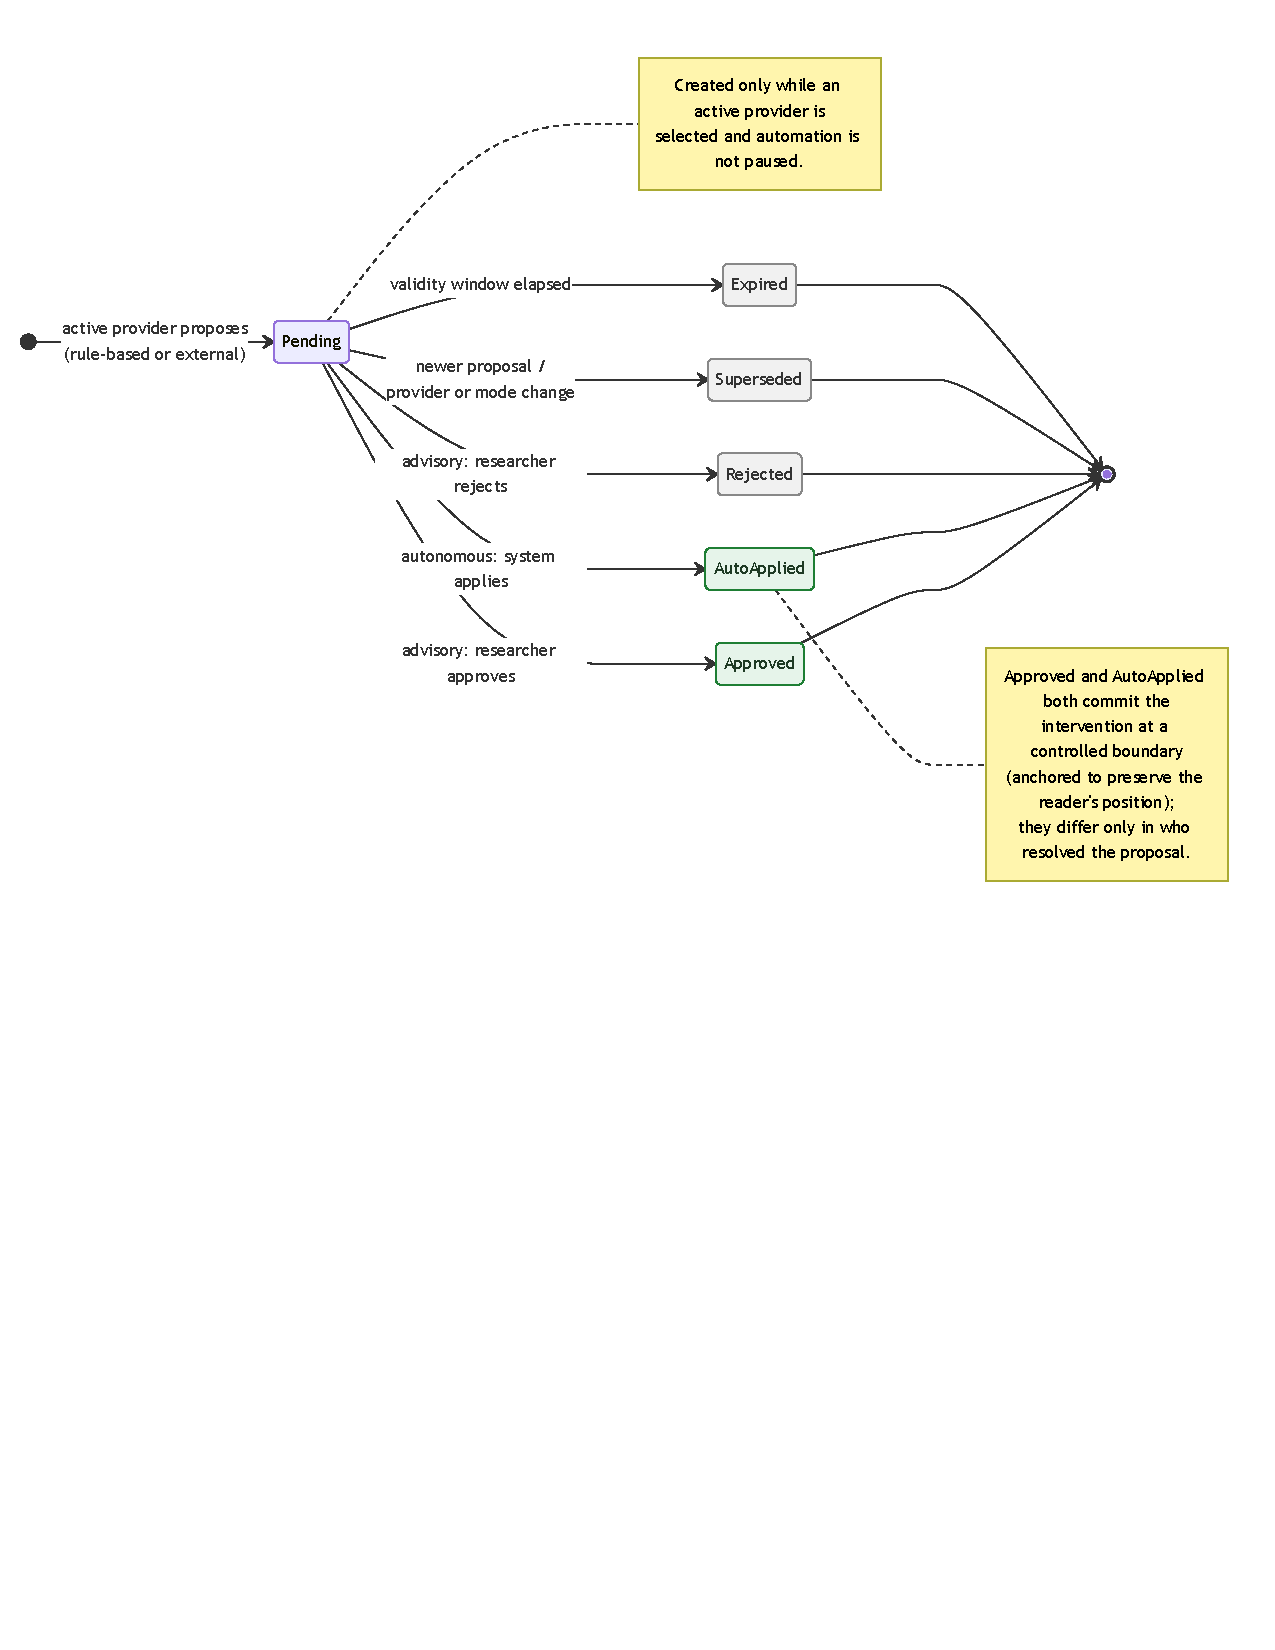
\includegraphics[width=\linewidth]{Chapters/05_SystemDesign/decision-lifecycle.pdf}
\caption{Lifecycle of a decision proposal. A proposal raised by the active decision provider (built-in or external) enters a pending state and resolves into exactly one terminal outcome. The execution mode fixes who resolves it: in advisory mode the researcher approves or rejects the proposal, whereas in autonomous mode the platform applies it directly. Approval and autonomous application both commit the intervention at a controlled boundary and differ only in who resolved the proposal, while a proposal that is rejected or superseded by a newer one is discarded without altering the text.}
\label{fig:design-decision-lifecycle}
\end{figure}

Two properties of this lifecycle carry the operator-control argument that RQ4 examines.
First, approval and autonomous application reach the same committed intervention and differ only in who resolved the proposal, so the distinction between the modes is exactly the locus of human authority and nothing more, and in either mode the intervention is committed at the controlled boundary introduced above that preserves the reader's position (RQ3).
Second, a pending proposal that is overtaken by a newer one, or invalidated by a change of provider or of mode, is superseded rather than silently applied, so that the text never adapts on a decision that no longer holds.
The lifecycle reserves a further terminal outcome, expiry, for a pending proposal whose window of validity has elapsed, on the same principle that a proposal is valid only while the signal that triggered it still describes the reader; the domain defines this state and permits the transition, but the present runtime does not yet drive it automatically, so a validity-window timer remains a designed extension point rather than an implemented trigger.
Because every proposal and its resolution are stamped into the session record of \cref{sec:design-data}, the mode in force and the fate of each proposal are themselves reproducible, which is what makes the researcher's control auditable after the session rather than merely exercised during it.

Because a reading session involves an invited participant and cannot be repeated cheaply, the loop is built to survive disturbance rather than to assume its absence.
It degrades gracefully: a client that disconnects falls out of the broadcast without interrupting the stream, and a decision provider that returns nothing, or is not present, yields no proposal and the cycle continues unaffected.
It also checkpoints its state, so that an interrupted session is recoverable: every state-changing step writes a checkpoint while holding the session lock, and a background worker independently persists the session at a fixed interval and again at shutdown.
This checkpointing is best-effort by design, swallowing its own failures, so that the durability mechanism can never itself halt a running session (D3).

The loop continually emits events and state changes, and those that are checkpointed accumulate into a record of the session.
That record is not merely a recovery aid but the platform's primary research output, and \cref{sec:design-data} turns from the live loop to the authoritative account it leaves behind.
